\begin{figure}[ht]
    \centering
    \subfigure[Initialization]{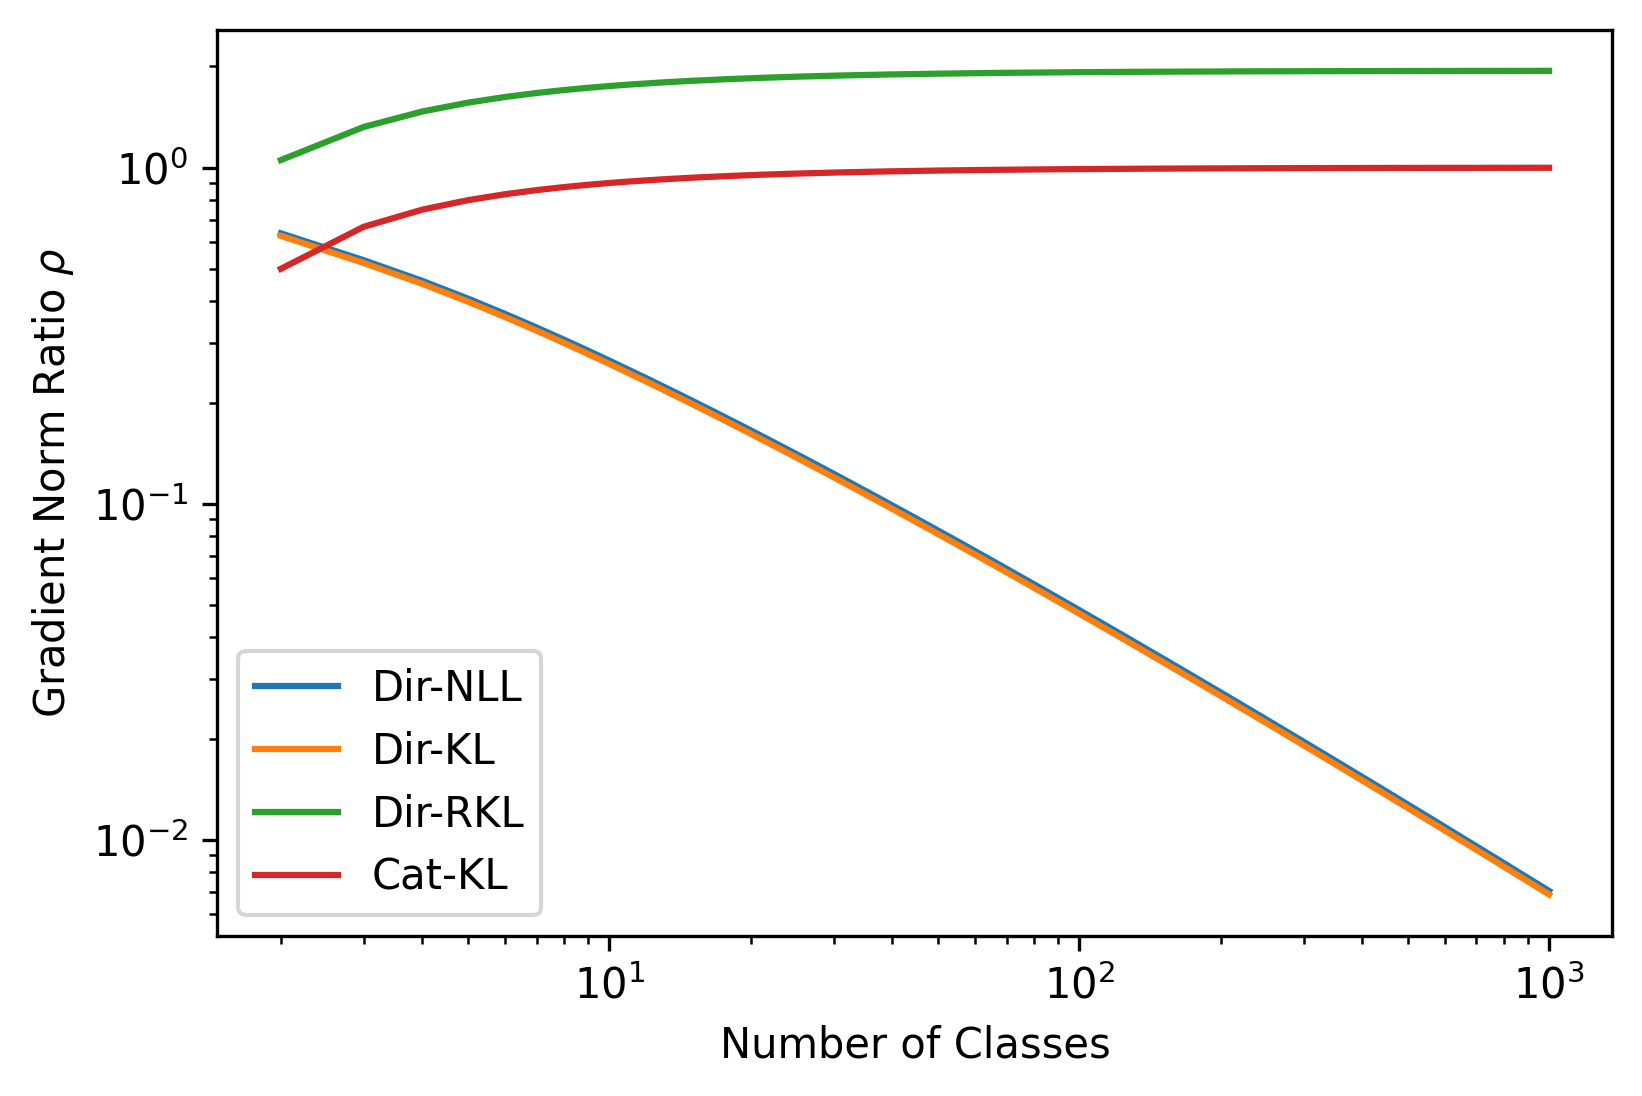
\includegraphics[width=0.32\textwidth]{figures/grad_ratio_init.png}}
    \subfigure[Near Convergence]{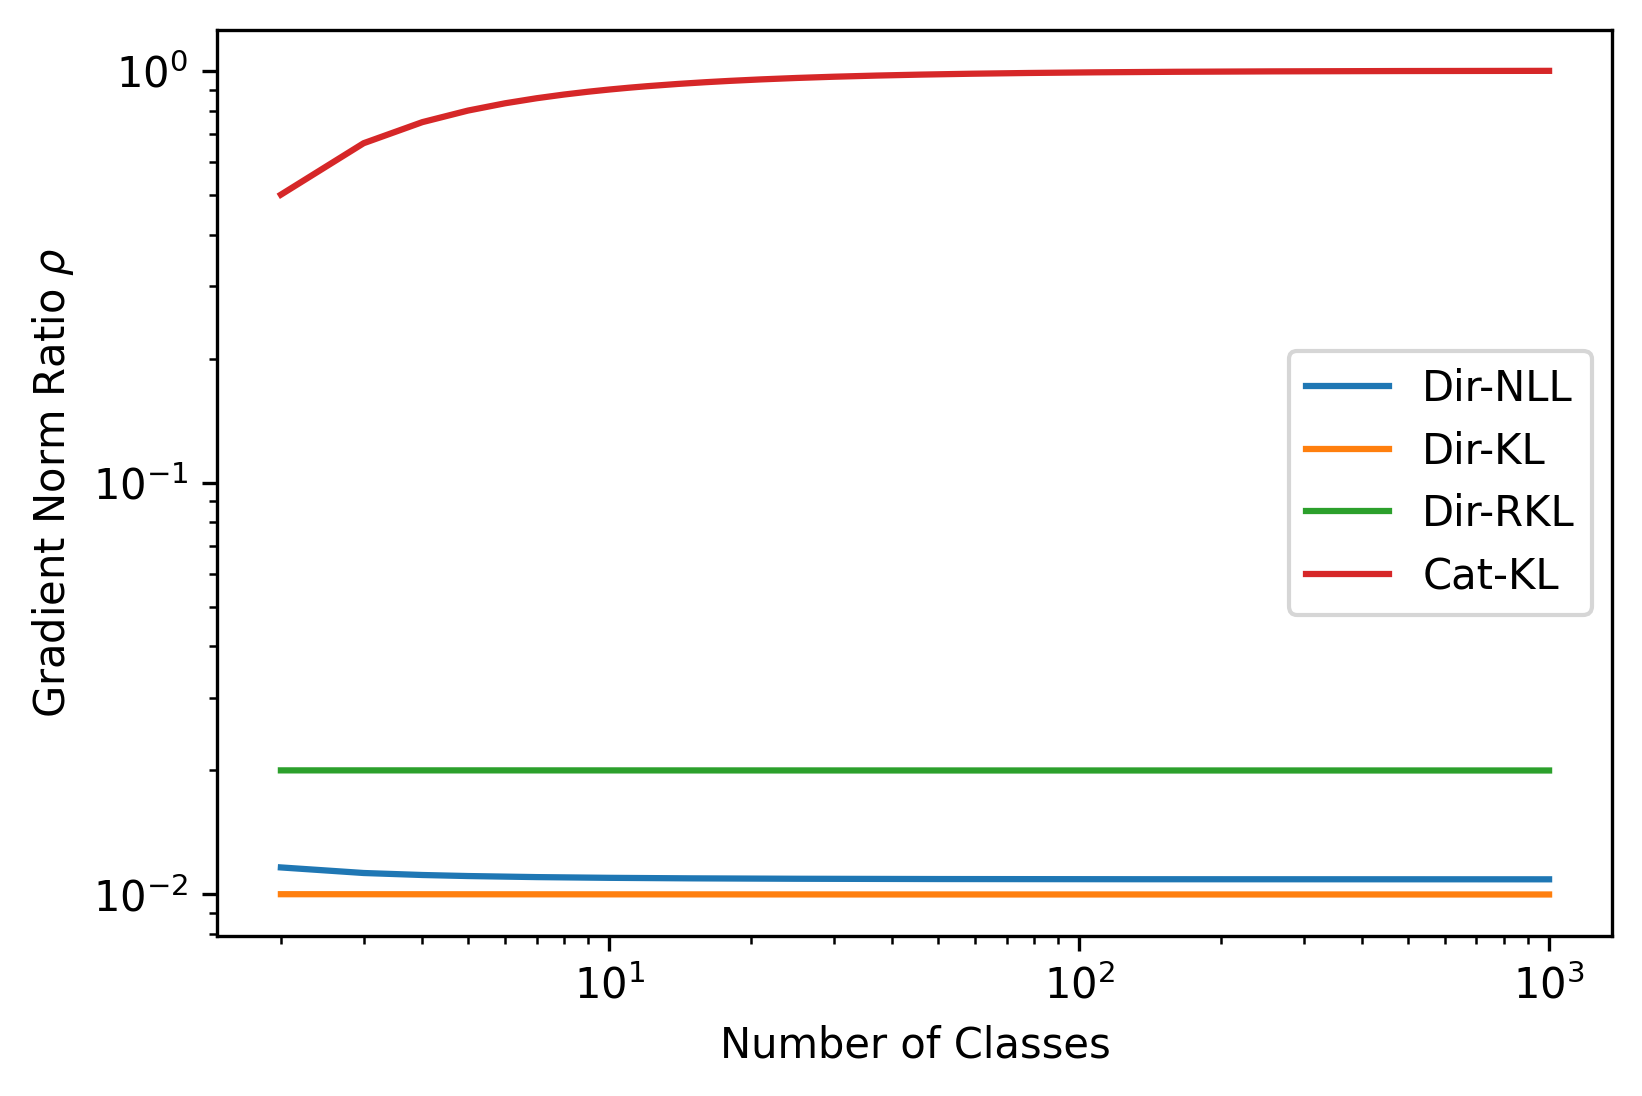
\includegraphics[width=0.32\textwidth]{figures/grad_ratio_conv.png}}
    \subfigure[Misclassification]{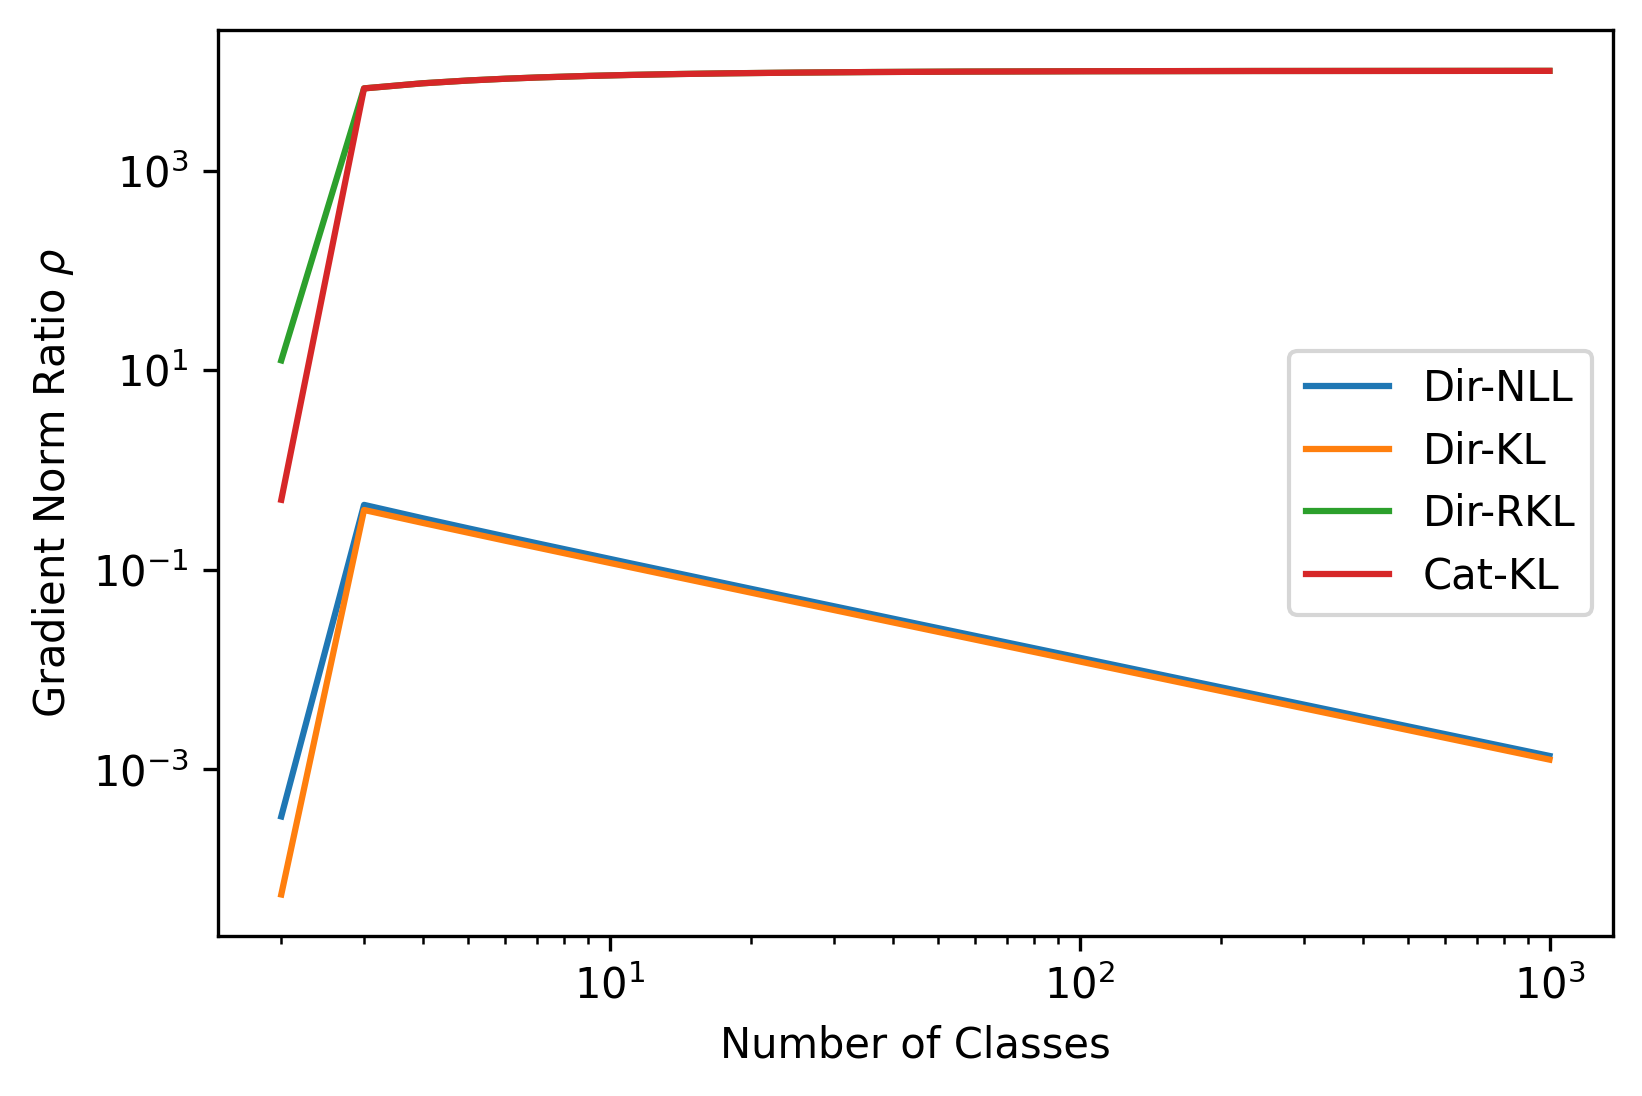
\includegraphics[width=0.32\textwidth]{figures/grad_ratio_misc.png}}
    \caption{Gradient Ratio}
    \label{fig:grad_ratio}
\end{figure}



\section{Theoretical Analysis and Alternative Loss functions}

In the previous section we described how \Endd can be done by maximising the log-likelihood of the ensemble's output distributions under a conditional Dirichlet Prior. However, we empirically observed significant convergence issues when applying this approach to tasks with large numbers of classes. Thus, in this section we examine the gradients of the Dirichlet NLL loss and propose an alternate training approach which overcomes them.


\textbf{First-Order Analysis}

The setup which will consider in our analysis is the following. First, we have a Prior Network model which is initialized such that it always returns a uniform Dirichlet distribution ($\bm{\alpha} = \bm{1}$), while the target distribution whose probability is being maximized is a sparse K-length vector of probabilities:
\begin{empheq}{align*}
    \bm{\pi}_{tgt} = \big[1-\epsilon, \epsilon/(K-1), \epsilon/(K-1), \cdots \big]^{\tt T},\quad \epsilon = \text{1e-4}
\end{empheq}
Second, we have a Prior Network which is \emph{near convergence} with the following output distribution:
\begin{empheq}{align*}
    \bm{\alpha}_{cnv} =&\ \bm{\pi}_{cnv} \cdot \alpha_0,\ \alpha_0 = 90K,\quad 
    \bm{\pi}_{cnv} =\ \big[1-5\epsilon, \frac{5\epsilon}{K-1}, \frac{5\epsilon}{K-1}, \cdots \big]^{\tt T}
\end{empheq}
Finally, we have a Prior Network which has made a strong mistake, which represents a situation which could occur somewhere in the middle on training, far from convergence:
\begin{empheq}{align*}
    \bm{\alpha}_{msc} =&\ \bm{\pi}_{msc} \cdot \alpha_0,\ \alpha_0 = 90K,\quad 
    \bm{\pi}_{msc} =\ \big[\frac{5\epsilon}{K-1}, \frac{5\epsilon}{K-1}, \cdots, 1-5\epsilon \big]^{\tt T}
\end{empheq}

First, lets consider the standard cross-entropy loss between a predicted and target discrete distribution and it's gradient with respect to the logit $z_k$:
\begin{empheq}{align}
    \mathcal{L}^{\text{CE}} =&\ -\sum_{k=1}^K \hat \pi_k \ln\big(\frac{\alpha_k}{\alpha_0}\big),\quad 
    \frac{\partial\mathcal{L}^{\text{CE}}}{\partial z_k} =\ \frac{\alpha_k}{\alpha_0} - \hat \pi_k 
\end{empheq}

Second, consider the NLL loss of a Dirichlet distribution and its gradient with respect to logit $z_k$:
\begin{empheq}{align}
   \mathcal{L} \small{=} \sum_{k=1}^K\Gamma(\alpha_k) \small{-}(\alpha_k \small{-} 1)\sum_{m=1}^M\frac{\ln\pi_k^{(m)}}{M} \small{-} \Gamma(\alpha_0), \   \frac{\partial\mathcal{L}}{\partial z_k} \small{=} \big(\psi(\alpha_k) \small{-} \psi(\alpha_0)  \small{-}\sum_{m=1}^M\frac{\ln\pi_k^{(m)}}{M}\big) \cdot \alpha_k
\end{empheq}

Finally, consider the dimensionality normalized ratio of the gradient with respect to the logit 1 and logit 2, which represents the relative contribution of the gradients with respect to the class we are interested in modelling to the long tail. 
\begin{empheq}{align}
\begin{split}
        \rho = \frac{1}{K} \Big| \frac{\partial\mathcal{L}}{\partial z_1} \Big| \Big/ \Big|\frac{\partial\mathcal{L}}{\partial z_2}\Big|
\end{split}
\end{empheq}
Figure~\ref{fig:grad_ratio} shows that, at initialization, as the number of classes is increased the standard cross-entropy loss primarily focuses on the high probability class and ignores the long tail. In contrast, the Dirichlet NLL loss displays a diminishing contribution. This means that the loss will focus on modelling the probability distribution of the high-probability classes only after it \emph{perfectly} models the long tail. As the loss is also very sensitive, it means that on complex tasks the model is perpetually stuck modelling the probabilities of tail classes. Note that even near convergence, the ratio $\rho$ is far smaller for the NLL criterion than for discrete cross-entropy. Finally, if a significant error is made on the training data, $\rho$ becomes very large for cross-entropy, and increasingly small for Dirichlet NLL as the number of classes increases. This analysis shows that a desirable property of the loss which ensures good convergence is that the ratio $\rho$ is high and either constant or increasing as the number of classes grows, otherwise the model focuses on modelling the distribution of tail-class probabilities across the ensemble.

An additional issue to consider is that the NLL noise is also noisy, as for each input $\bm{x}$ we only have a few discrete distributions - it may be necessary to use far more samples to get a good estimate of the ensemble's distribution. Furthermore, this distribution may be poorly matched to the Dirichlet, which introduces additional issues. Thus, a natural solution to consider would be to introduce a \emph{Proxy Dirichlet Distribution} to which we can minimize either the \emph{KL-divergence} or \emph{reverse KL divergence}. We leave discussion of the details of the Proxy Dirichlet until later and only consider the gradients which arise from minimizing either loss.  

For this analysis we consider a target Dirichlet distribution with parameters $\bm{\beta} = \bm{\pi}_{tgt}*\beta_0$ where $\beta_0 = 100K$. The explicit forms of the KL-divergence between two Dirichlet distributions, as well the gradient of the forward and reverse KL-divergence are provided below:
\begin{empheq}{align}
\begin{split}
       & \mathcal{L}^{\text{KL}} =\ \ \sum_{k=1}^K\Gamma(\alpha_k) - \sum_{k=1}^K\Gamma(\beta_k) + \Gamma(\beta_0) - \Gamma(\alpha_0) + \sum_{k=1}^K(\beta_k - \alpha_k)\Big(\psi(\beta_k)-\psi(\beta_0)\Big)
\end{split} \\
\begin{split}
       & \mathcal{L}^{\text{RKL}} =\ \ \sum_{k=1}^K\Gamma(\beta_k) - \sum_{k=1}^K\Gamma(\alpha_k) + \Gamma(\alpha_0) - \Gamma(\beta_0) + \sum_{k=1}^K(\alpha_k - \beta_k)\Big(\psi(\alpha_k)-\psi(\alpha_0)\Big)
\end{split} \\
\begin{split}
        &\frac{\partial\mathcal{L}^{\text{KL}}}{\partial z_k} =\ \big(\psi(\alpha_k) - \psi(\alpha_0) - \psi(\beta_k) + \psi(\beta_0)\big) \cdot \alpha_k
\end{split} \\
\begin{split}
        &\frac{\partial\mathcal{L}^{\text{\tiny RKL}}}{\partial z_k} =\ \big((\alpha_k - \beta_k)\psi'(\alpha_k) - (\alpha_0 - \beta_0)\psi'(\alpha_0)\big) \cdot \alpha_k
\end{split}
\end{empheq}

Figure~\ref{fig:grad_ratio} additionally displays the ratio $\rho$ for both the forward and reverse KL-divergence losses. The forward KL-divergence displays the same issues as the NLL loss and $\rho$ continues to decrease as the number of classes in increased. This is unsurprising, as the NLL is equivalent to the KL-divergence in the limit. However, the \emph{reverse KL-divergence} displays the desirable properly that $\rho$ grows and stabilizes as the number of classes is increased. This suggests that if we were to minimize the \emph{reverse KL-divergence} to an appropriately chosen \emph{Proxy-Target Dirichlet distribution}, then we would be able to avoid convergence issues. 

% \textbf{Second-Order Analysis}

% In addition to the first-order analysis provided above, we also conduct a second order analysis by considering the eigenvalues of the Hessian of the loss.


\textbf{Proxy-Dirichlet distribution}

\begin{figure*}[ht]
    \centering
    \subfigure[Naive \Endd]{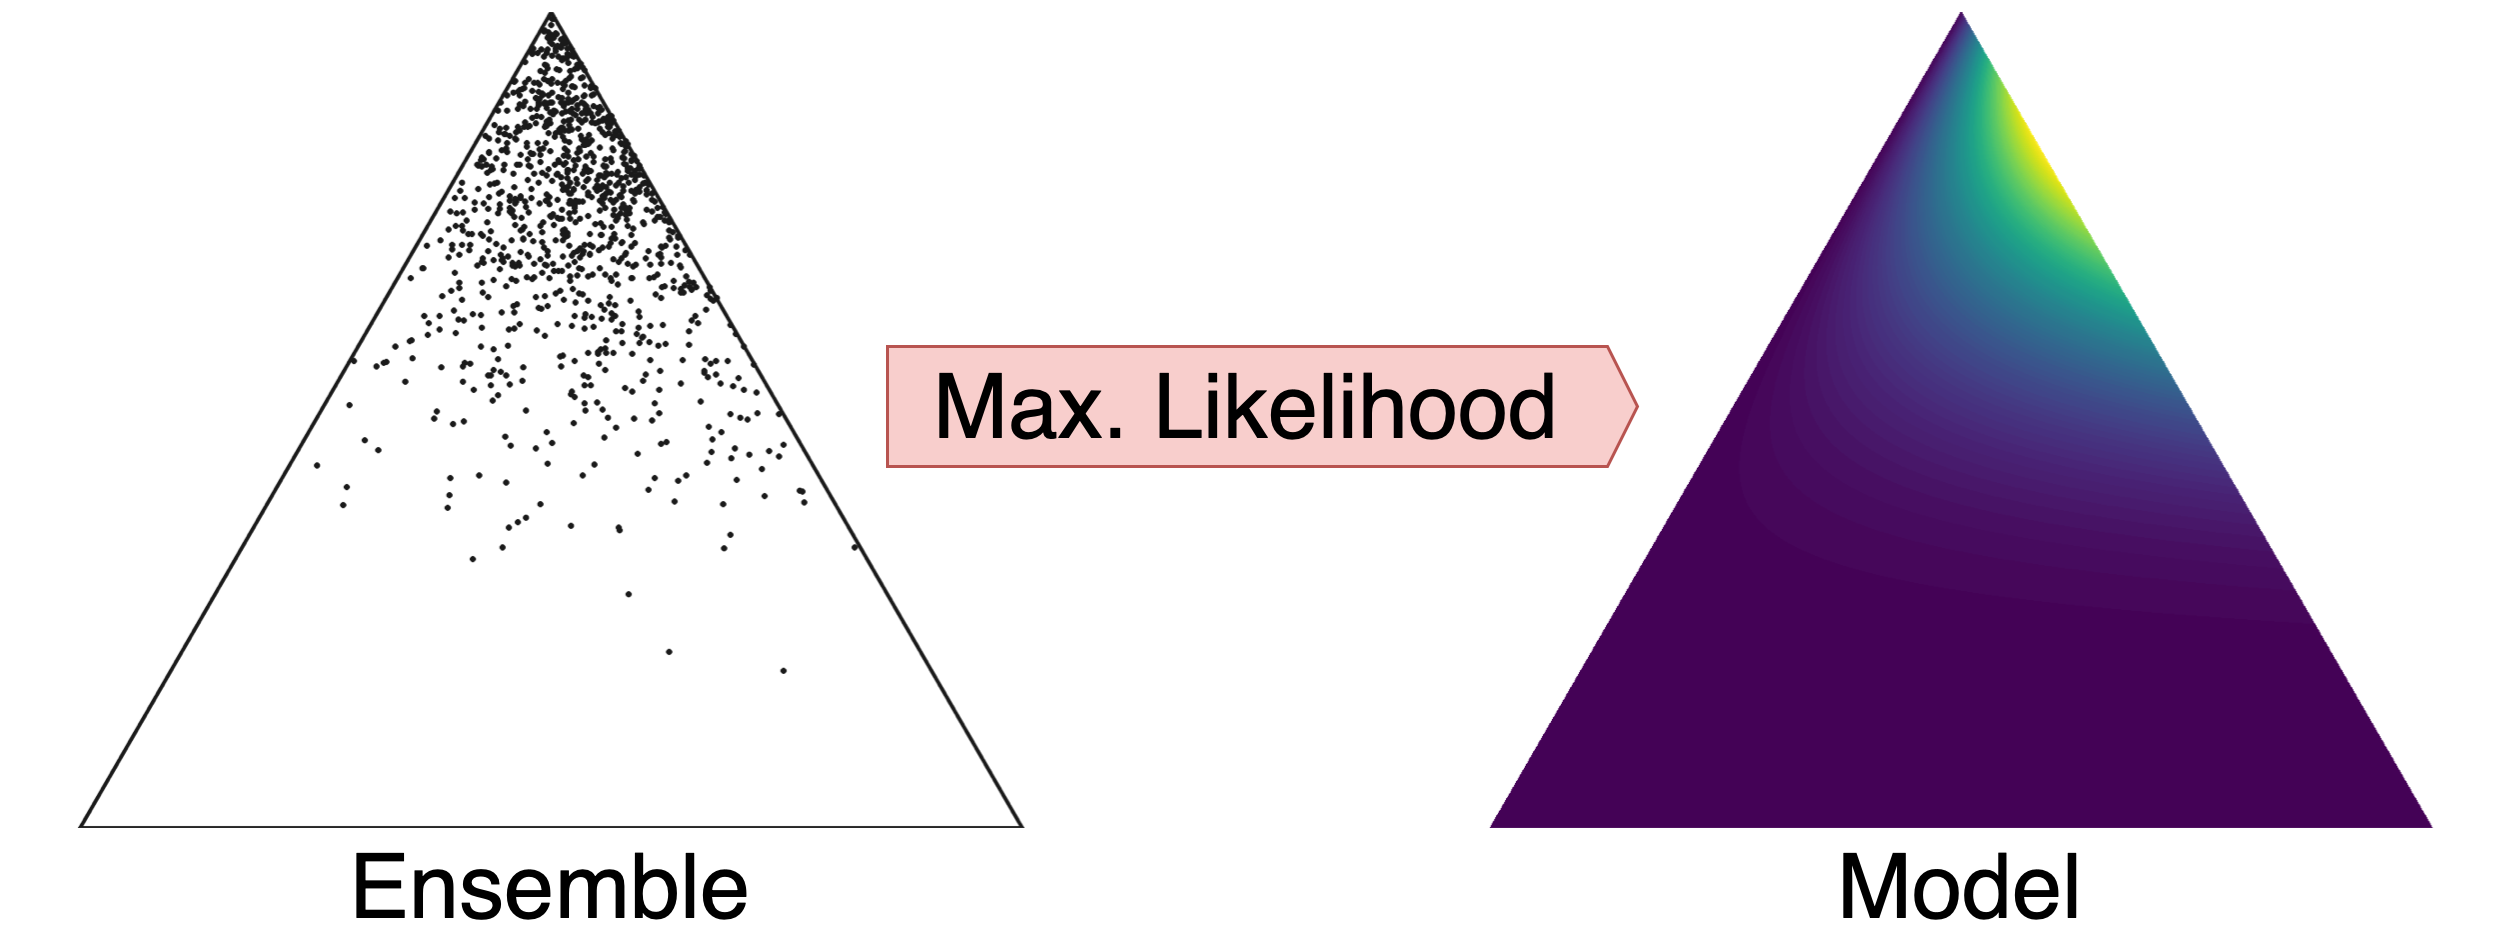
\includegraphics[scale=0.067]{figures/naive-distillation-2.png}}
    \subfigure[Proxy \Endd]{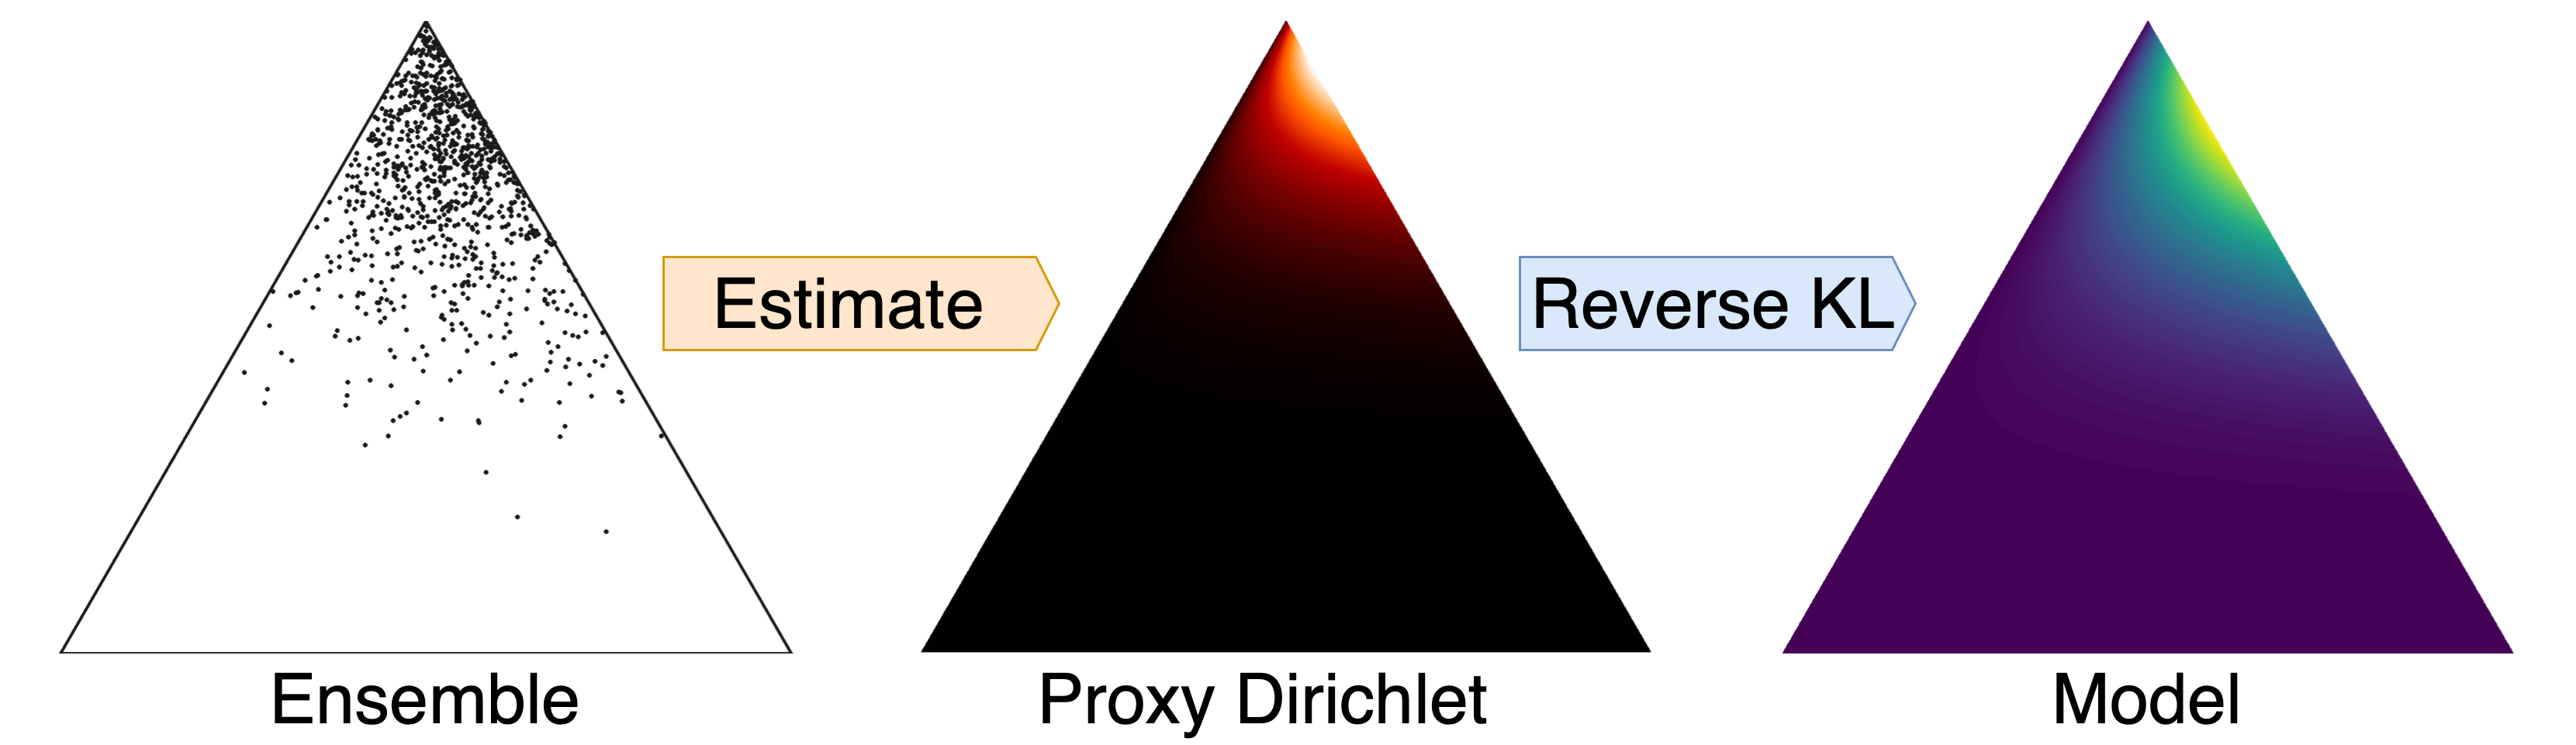
\includegraphics[scale=0.067]{figures/proxy_distillation.png}}
    \caption{Schematic of Distillation Approaches}
    \label{fig:distillation overview}
\end{figure*}

It is important to remember that the ensemble may be poorly modelled via a Dirichlet distribution, so it is necessary to ask which properties of the ensemble we are actually interested in capturing. Clearly, we would like to capture the mean of the ensemble, as that typically has better predictive accuracy and calibration. Additionally, we would like to capture \emph{bulk-diversity properties} of the ensemble, such that the measures of divergence derived from the Proxy Dirichlet are similar to those of the original ensemble and therefore provide a similar rank-ordering of data. At the same time, we are \emph{not} interested modelling properties like multi-modality and skew. 

Clearly, obtaining the mean of the ensemble is trivial. Obtaining an estimate of the precision $\beta_0$ is more challenging. One approach based on Sterling's approximation is described in~\cite{minka2000estimating} and proposes the following estimate:
\begin{empheq}{align}
\begin{split}
        \hat \pi_k (\bm{x})=&\ \frac{1}{M}\sum_{m=1}^M {\tt P}(y=\omega_k|\bm{x}, \bm{\theta}^{(m)}) \\
        \tilde \beta_0(\bm{x}) =& \frac{K-1}{2 \sum_{k=1}^K\hat \pi_k (\ln \hat \pi_k - \frac{1}{M}\sum_{m=1}^M\ln \pi_k^{(m)})},\ \bm{\beta}_k (\bm{x}) = \ \hat \pi_k(\bm{x}) \cdot \tilde \beta_0(\bm{x}) + 1
\end{split}
\end{empheq}

We found that it is important to also add 1 to all the target concentration parameters. Figure~\ref{fig:grad_ratio_smooth} shows that for the reverse KL loss, adding 1 to \emph{both} the target Proxy-Dirichlet as well as \emph{the model} yields an improved ratio $\rho$ both at initialization and near convergence. Heuristically, it seems to make the loss more linear and stable by preventing the digamma and trigamma functions $\psi$ and $\psi'$ in the reverse-KL loss from dropping into the highly non-linear regime when $\alpha_k < 1$ and $\beta_k < 1$.
\begin{figure}[ht]
    \centering
    \subfigure[Initialization]{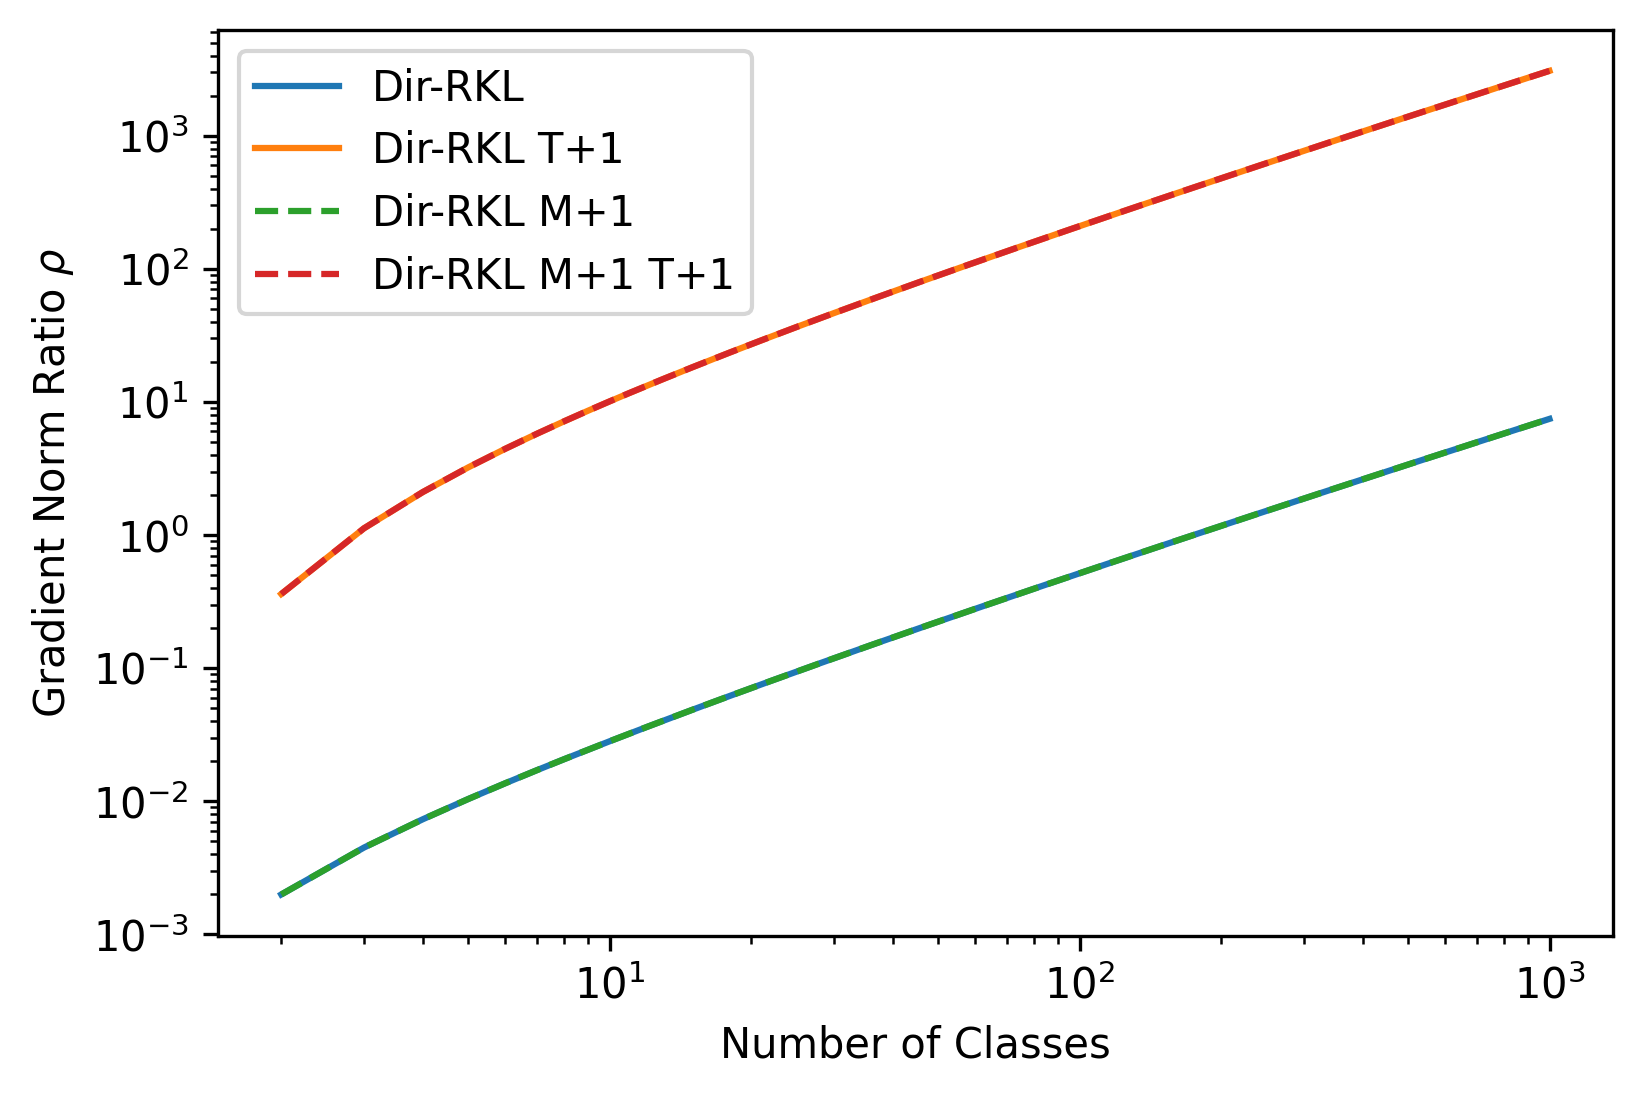
\includegraphics[scale=0.49]{figures/grad_ratio_init_smooth.png}}
    \subfigure[Near Convergence]{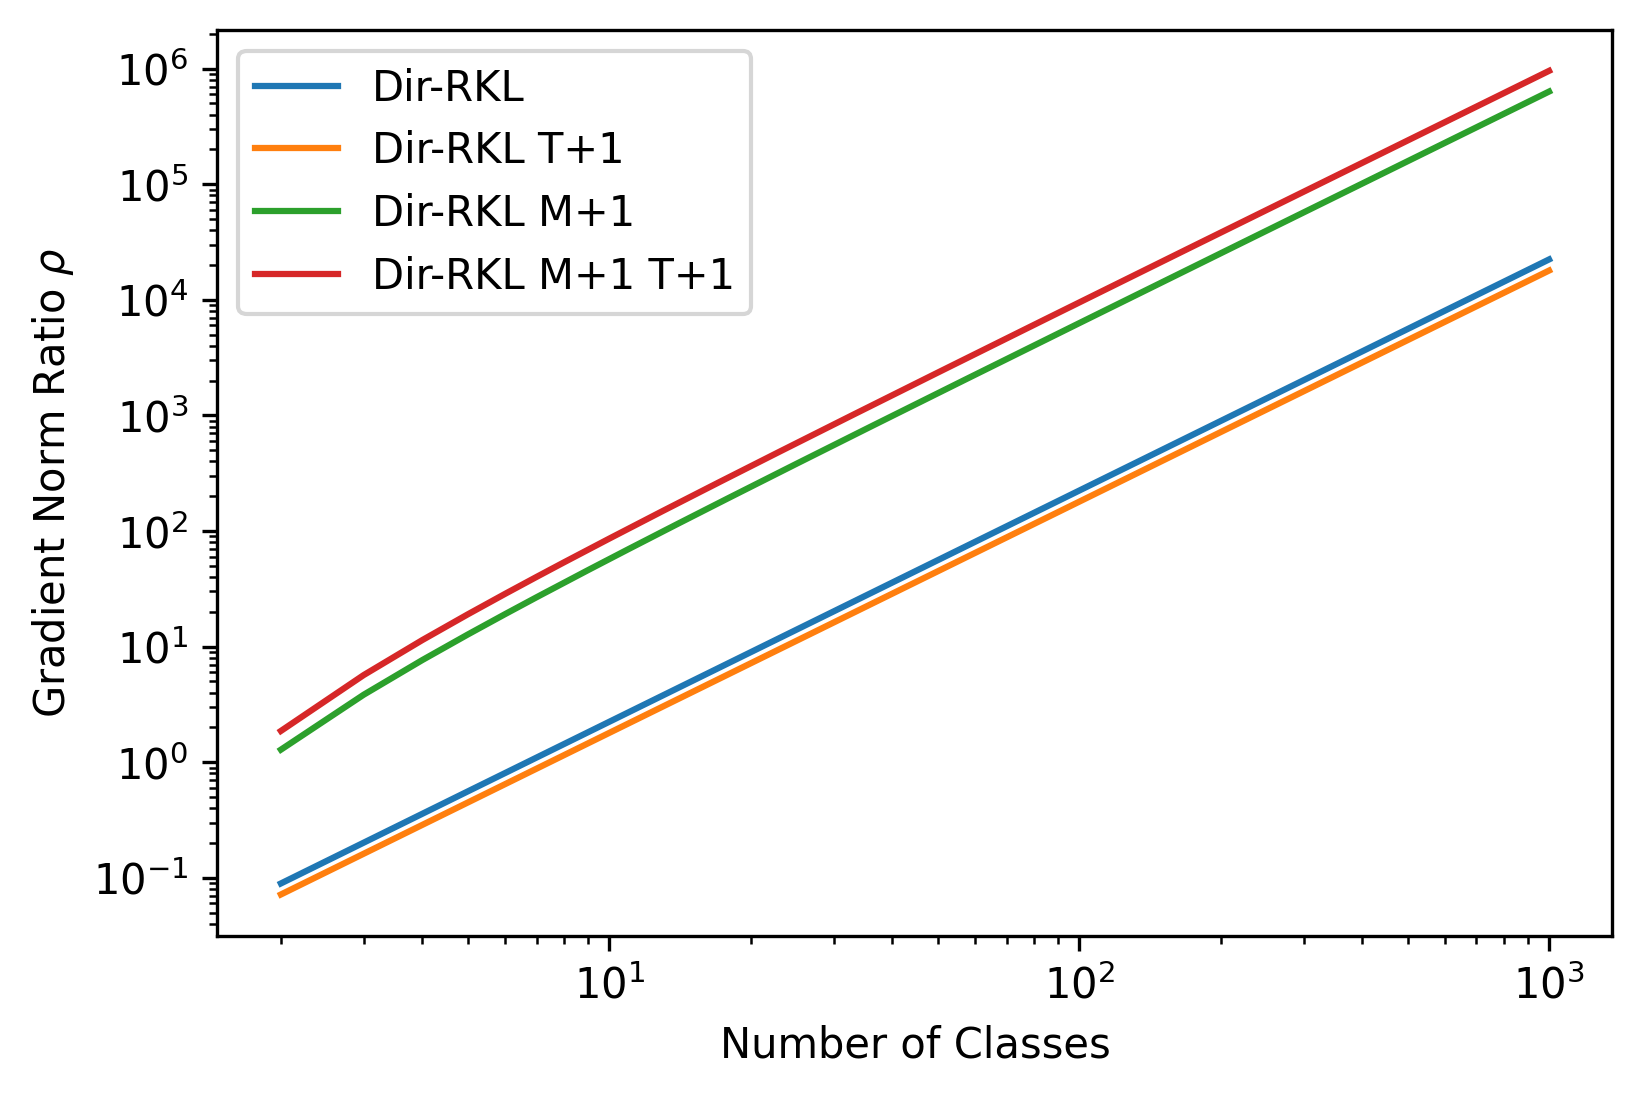
\includegraphics[scale=0.49]{figures/grad_ratio_conv_smooth.png}}
    \caption{Gradient Ratio}
    \label{fig:grad_ratio_smooth}
\end{figure}

Note, while the solution may seem to similar to work done in \cite{malinin-rkl-2019}, the fundamental underlying reason for using this loss is altogether different. Here, the issue is due to large gradients from low-probability tail classes, while in~\cite{malinin-rkl-2019} the reverse KL loss is used to avoid inducing a multi-modal target Dirichlet distribution in expectation. 

\begin{empheq}{align}
\begin{split}
{\tt KL}[{\tt p}(\bm{\pi}|\bm{x},\bm{\theta}) \| {\tt p}(\bm{\pi}|\bm{\hat \beta})] =&\ \underbrace{ \beta_0\cdot\mathbb{E}_{{\tt p}(\bm{\pi}|\bm{x},\bm{\theta})}\big[-\sum_{k=1}^K\hat \pi_k\ln \pi_k\big]}_{\text{Reconstruction term}} + \underbrace{{\tt KL}[{\tt p}(\bm{\pi}|\bm{x},\bm{\theta}) \| {\tt p}(\bm{\pi}|\bm{1})]}_{\text{Prior}} +Z
\end{split}
\end{empheq}
% \textbf{Alternative solutions (if it fits) }

% If not, we'll move that to the appendix (along with comparisons)

% \begin{itemize}
%     \item Top-k aggregation
%     \item Softplus parametrization
% \end{itemize}